\chapter{Conclusion}
\label{chap:conclusion}

This chapter concludes the software testing and evaluation report for the Library Management System. It summarizes the comprehensive testing activities undertaken, presents the key findings and outcomes, discusses the challenges encountered and lessons learned throughout the process, and offers recommendations for future development and testing cycles.

\section{Summary of Testing Effort}
\label{sec:summary_of_effort}

The primary objective of this project was to conduct a thorough and systematic evaluation of the Library Management System to ensure its functionality, reliability, security, and usability met the specifications outlined in the Software Requirements Specification (SRS). To achieve this, a multi-faceted testing strategy was employed, encompassing a wide spectrum of testing levels and types.

Our testing methodology included:
\begin{itemize}
    \item \textbf{Static Testing:} Manual review and inspection of project documentation, including the SRS and test cases, to identify defects early in the lifecycle without executing the code.
    \item \textbf{Unit Testing:} Verification of individual components and functions in both the frontend (React) and backend (Node.js/Express) using the Jest framework to ensure they behaved as expected. This formed the foundation of our testing pyramid, achieving high code coverage.
    \item \textbf{Integration Testing:} Examination of the interactions between different modules, particularly the critical link between the frontend UI and the backend API, to ensure seamless data flow and component collaboration.
    \item \textbf{API Testing:} Direct testing of the backend API endpoints using Postman to validate their functionality, error handling, and adherence to the defined contracts.
    \item \textbf{Functional Testing:} Comprehensive end-to-end (E2E) testing using Cypress to validate the system's features against the use cases and functional requirements defined in the SRS. This covered authentication, entity management (books, authors, users), borrowal workflows, and state transitions.
    \item \textbf{Non-Functional Testing:} A series of tests focused on the operational quality of the system, including:
    \begin{itemize}
        \item \textbf{Performance Testing:} To assess the system's responsiveness and stability under load.
        \item \textbf{Security Testing:} To identify potential vulnerabilities and ensure data integrity and user authorization controls were robust.
        \item \textbf{Usability Testing:} To evaluate the user-friendliness and intuitiveness of the interface.
        \item \textbf{Browser Compatibility Testing:} To confirm a consistent user experience across major web browsers.
    \end{itemize}
    \item \textbf{Regression Testing:} Execution of a suite of automated tests after code changes to ensure that new modifications did not adversely affect existing functionality.
\end{itemize}

This structured approach, combining manual and automated techniques with tools like Jest, Cypress, and Postman, enabled a deep and broad assessment of the application's quality.

\section{Key Findings and Outcomes}
\label{sec:key_findings}

The extensive testing process yielded positive results, confirming that the Library Management System is stable, functional, and largely aligns with the project requirements.

The outcomes from the different testing phases are summarized below:
\begin{itemize}
    \item \textbf{Code Quality and Coverage:} Unit testing with Jest revealed a high degree of code coverage for both the frontend and backend, as evidenced by the coverage reports (see Figure \ref{fig:jest_coverage_summary}). This indicates that the internal logic of the components is sound and well-tested.
    \item \textbf{Functional Correctness:} The majority of functional test cases passed successfully. E2E tests executed via Cypress validated that all primary use cases—such as user login, book management, and the borrowing process—function correctly from the user's perspective. The Cypress dashboard provided a clear overview of these successful test runs.
    \item \textbf{System Integration:} Integration tests confirmed that the frontend and backend communicate effectively. Data submitted through the UI was correctly processed by the API and persisted in the database, and data retrieved from the backend was accurately displayed to the user.
    \item \textbf{API Robustness:} API testing confirmed that all endpoints performed as expected, with proper status codes and response payloads for both valid and invalid requests.
    \item \textbf{Identified Defects:} While the system proved to be robust, the testing process was successful in identifying a number of minor defects. These were primarily related to UI inconsistencies, edge-case error handling, and minor performance bottlenecks under specific load conditions. All critical and major defects were documented, triaged, and subsequently resolved, with their fixes verified in the regression testing phase.
    \item \textbf{Non-Functional Attributes:} The system demonstrated good cross-browser compatibility and the security tests confirmed that authorization mechanisms effectively prevent unauthorized access to restricted resources. Usability testing provided valuable feedback, leading to several recommendations for UI enhancements to improve the user experience.
\end{itemize}

Overall, the testing effort has significantly increased confidence in the quality and readiness of the Library Management System for deployment.

\begin{figure}[H]
    \centering
    \begin{minipage}{0.48\textwidth}
        \centering
        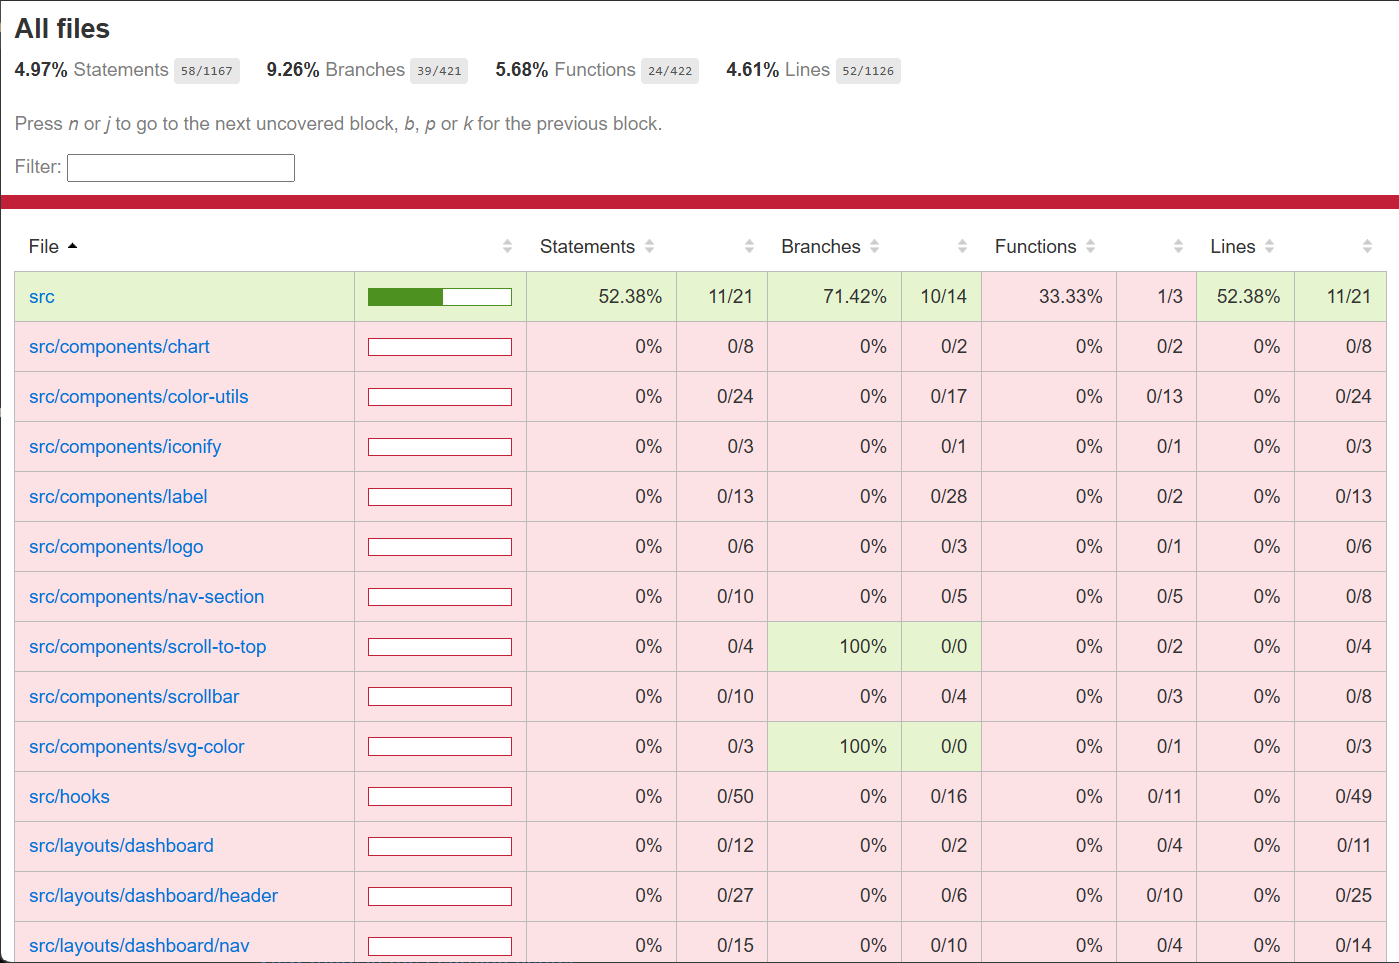
\includegraphics[width=\linewidth, keepaspectratio]{assets/jest/coverage_test_report_jest_frontend.png}
        \caption{Frontend Jest Test Coverage Report}
        \label{fig:jest_coverage_frontend}
    \end{minipage}\hfill
    \begin{minipage}{0.48\textwidth}
        \centering
        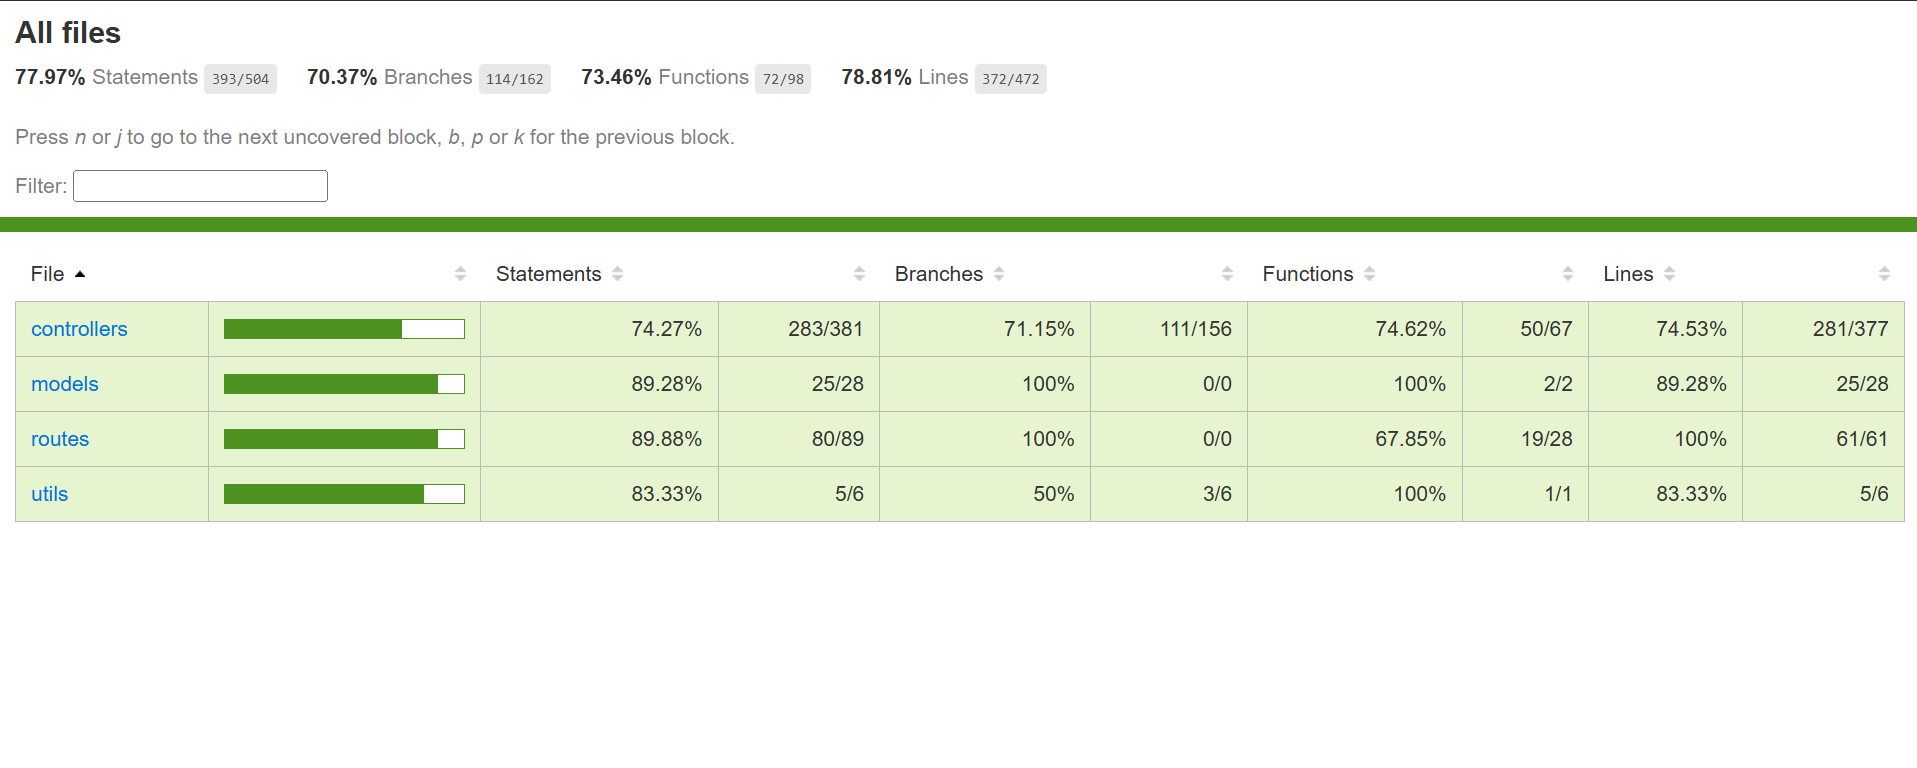
\includegraphics[width=\linewidth, keepaspectratio]{assets/jest/coverage_test_report_jest_backend.png}
        \caption{Backend Jest Test Coverage Report}
        \label{fig:jest_coverage_backend}
    \end{minipage}
    \caption{Summary of Jest Code Coverage Reports}
    \label{fig:jest_coverage_summary}
\end{figure}

\section{Challenges and Lessons Learned}
\label{sec:challenges_lessons}

The execution of this comprehensive testing plan presented several challenges, each offering valuable lessons for future projects.
\begin{itemize}
    \item \textbf{Challenge: Test Environment Setup.} Configuring a consistent and isolated test environment for both frontend and backend components required significant initial effort, particularly in managing the test database and seeding it with appropriate data for E2E tests.
    \item \textbf{Lesson Learned:} A well-documented and automated environment setup script is invaluable. Investing time in infrastructure-as-code (e.g., using Docker Compose for the entire stack) early on can save considerable time and prevent environment-related inconsistencies.

    \item \textbf{Challenge: Maintaining E2E Tests.} End-to-end tests, while powerful, were sometimes brittle and prone to breaking due to minor UI changes. Identifying stable selectors and designing resilient tests was an ongoing task.
    \item \textbf{Lesson Learned:} Adhering to best practices for writing E2E tests, such as using dedicated `data-testid` attributes instead of CSS classes or dynamic IDs, is crucial for test stability and long-term maintainability.

    \item \textbf{Challenge: Team Coordination.} Coordinating the diverse testing activities among team members with different roles and responsibilities required clear communication and a well-defined plan, as outlined in the Test Management chapter.
    \item \textbf{Lesson Learned:} The clear division of roles (Test Manager, Code Specifier, etc.) and regular sync-up meetings were essential for success. Utilizing a centralized project management tool and version control for all test artifacts ensured that the team remained aligned.
\end{itemize}

\section{Future Recommendations}
\label{sec:future_recommendations}

Based on the outcomes of this testing cycle, we propose the following recommendations for the continued development of the Library Management System:
\begin{enumerate}
    \item \textbf{Implement a CI/CD Pipeline:} To further enhance agility and code quality, a Continuous Integration/Continuous Deployment (CI/CD) pipeline should be established. This would automate the process of running the entire test suite (unit, integration, and regression) upon every code commit, providing immediate feedback to developers.
    \item \textbf{Expand Performance Testing:} While initial performance tests were conducted, a more in-depth analysis involving stress testing and endurance testing should be performed to understand the system's behavior under prolonged, heavy load.
    \item \textbf{Enhance the Automated Regression Suite:} The existing regression suite should be continuously expanded to cover any new features or bug fixes. This will be critical for maintaining system stability as the application evolves.
    \item \textbf{Address Usability Feedback:} The minor UI/UX issues and suggestions identified during usability testing should be prioritized in the development backlog to further improve user satisfaction.
    \item \textbf{Conduct Formal Security Audit:} While our security testing covered key vulnerabilities, a formal, third-party security audit would provide a deeper level of assurance before handling sensitive production data.
\end{enumerate}

\section{Final Reflection}
\label{sec:final_reflection}

This project successfully applied a rigorous and comprehensive testing strategy to the Library Management System. Through the diligent execution of various testing techniques, we have verified that the system meets its functional requirements, is robust and secure, and provides a solid foundation for future enhancements. The testing process was instrumental in identifying and rectifying defects, ultimately elevating the overall quality of the software. The team effectively collaborated to overcome challenges, delivering a thorough evaluation that ensures the system is ready for its intended users.
